\chapter{Experimental Results}
In this chapter, the testbed is used for evaluation of various standard RL algorithms for vision based robot manipulation tasks.

\section{Simulator performance}
The simulation environment can be run in following configurations

\begin{itemize}
	\item Realtime mode - Simulation is run at realtime with rendering ON
	\item Fast rendering mode - Simulation is run rendering turned on but not at realtime
	\item Fast non rendering mode - Simulation is run with rendering and realtime turned OFF
\end{itemize}

The metric used for measuring performance of simulator is action time. Action time is the time taken by the simulator to execute a particular action

\begin{figure}
	\caption{Simulator performance at different modes (Mode vs Mean Action Time)}
	\centering
	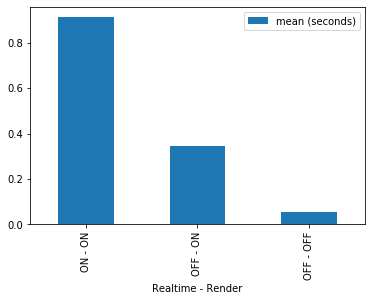
\includegraphics[scale=0.7]{benchmark-table-clearing.png}
\end{figure}

\begin{table}
	\caption{Simulator performance (Mean action time in seconds) at different modes}
	\begin{tabular}{|c|c|c|c|c|c|c|c|}
		\hline
		\textbf{Render | Realtime} & \textbf{Mean} & \textbf{Std} & \textbf{Min} & \textbf{25\%} & \textbf{50\%} & \textbf{75\%} & \textbf{Max} \\
		\hline
		ON | ON & 0.912 & 2.783 & 0.138 & 0.358 & 0.374 & 0.39 & 26.33 \\
		\hline
		ON | OFF & 0.345 & 0.583 & 0.0793 & 0.198 & 0.206 & 0.214 & 4.342 \\
		\hline
		OFF | OFF & 0.053 & 0.023 & 0.041 & 0.046 & 0.047 & 0.048 & 0.201 \\
		\hline
	\end{tabular}
\end{table}

\section{Table clearing environment}
After training PPO agent on table clearing environment using 8 core 42GB RAM Nvidia T4 GPU system for 4M timesteps, results are shown below

\begin{figure}[H]
	\centering
	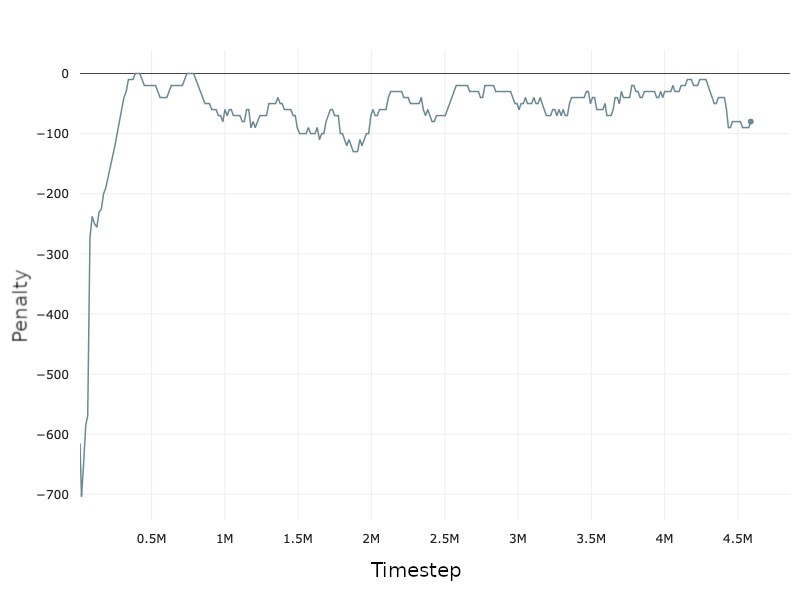
\includegraphics[scale=1]{ppo-simulation-collision-penalty}
	\caption{Collision penalty. Optimum value is 0}
\end{figure}

\begin{figure}[H]
	\centering
	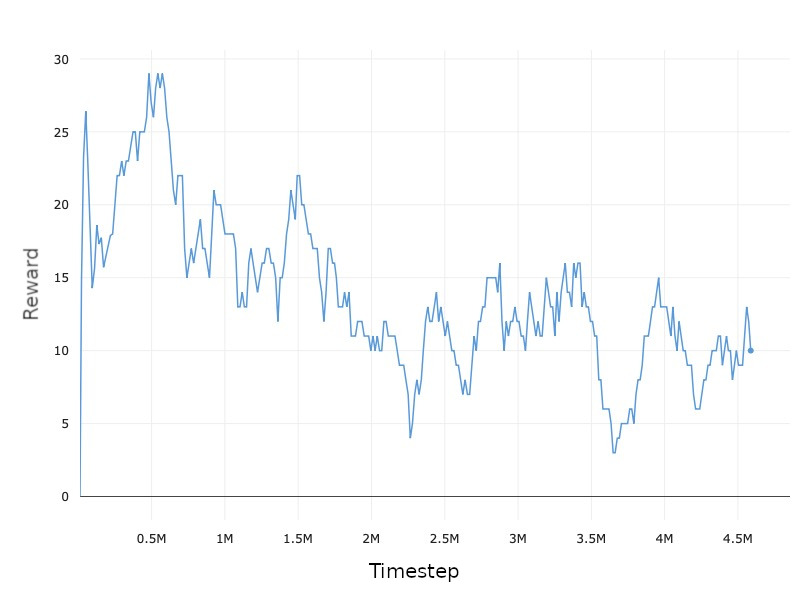
\includegraphics[scale=1]{ppo-simulation-grasp-reward}
	\caption{Grasp reward. Optimum value is 100}
\end{figure}

\begin{figure}[H]
	\centering
	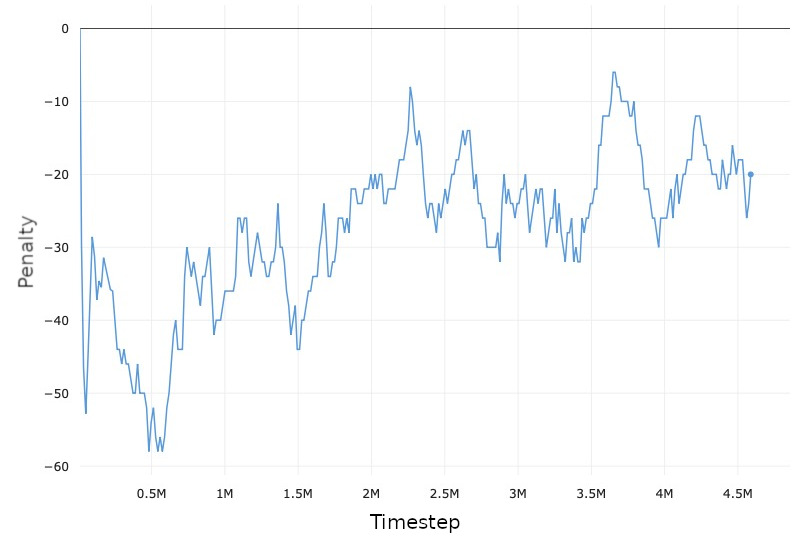
\includegraphics[scale=1]{ppo-simulation-drop-penalty}
	\caption{Drop penalty. Optimum value is 100}
\end{figure}

\begin{figure}[H]
	\centering
	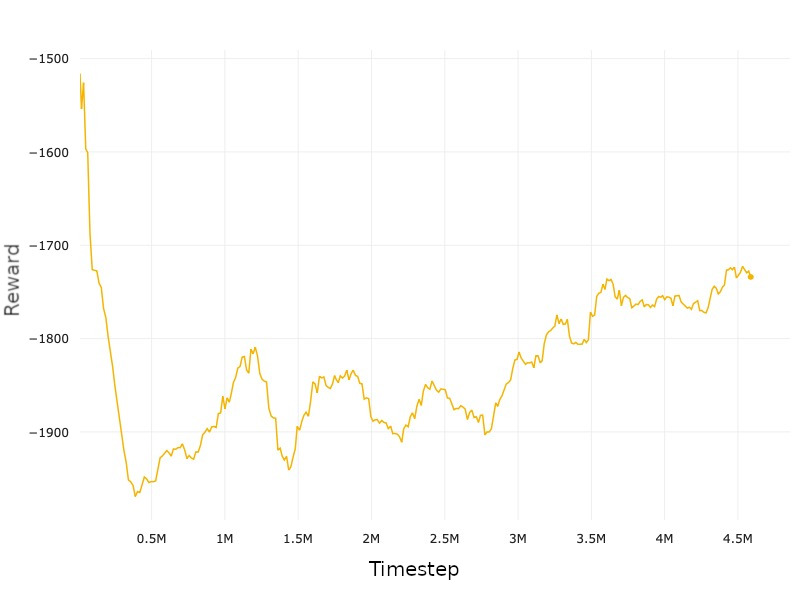
\includegraphics[scale=1]{ppo-simulation-reward-mean}
	\caption{Mean episode reward. Optimum value $\ge 200$}
\end{figure}

For attaining optimum reward, network needs to be trained for approximately 80M timesteps.